\documentclass[12pt]{mwart}

\usepackage{polski}
\usepackage[utf8]{inputenc}
\usepackage{mathtools,amsthm,amssymb,icomma,upgreek,xfrac, graphics, scrextend, float, hyperref}
\usepackage[table,xcdraw]{xcolor}
\mathtoolsset{mathic}
\raggedbottom
\graphicspath{ {./images/} }

\author{Mateusz Stasiak}
\title{Analiza danych rzeczywistych}


\begin{document}
\maketitle





\section{Wstęp}
\noindent Celem ćwiczenia jest analiza, porównanie i wizualizacja danych rzeczywistych przy pomocy metod statystyki opisowej. \\





\section{Pierwszy zestaw danych}
\subsection{Wprowadzenie}
\noindent Dane zostały pozyskane ze strony internetowej \url{https://vincentarelbundock.github.io/Rdatasets/datasets.html}. Dotyczą zarobków w Stanach Zjednoczonych w latach $1988-1989$. Składają się z $4266$ obserwacji. Każdej z nich przypisano roczną pensję w dolarach oraz odpowiednią grupę wiekową:
\begin{itemize}
	\item g1 - od $23$ do $26$ lat,
	\item g2 - od $27$ do $29$ lat,
	\item g3 - od $30$ do $32$ lat.
\end{itemize}

\begin{figure}[H]
	\begin{center}
	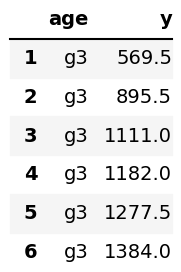
\includegraphics[scale=0.6]{head.png}
	\caption{Przykładowe dane}
	\end{center}
\end{figure}




\subsection{Analiza danych}
\noindent Efektywne opracowanie powyższych danych wymaga rozpatrywania każdej grupy wiekowej osobno.

\begin{figure}[H]
	\begin{center}
	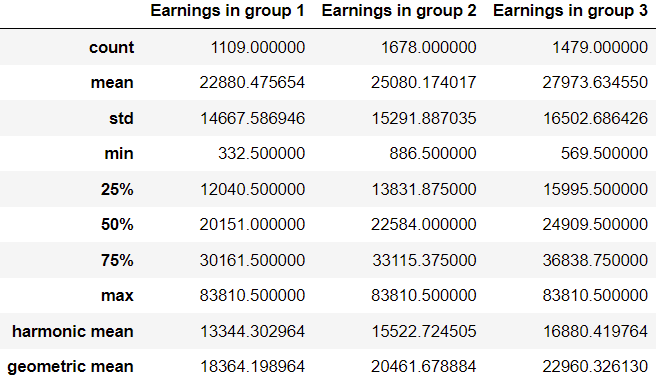
\includegraphics[scale=0.7]{compared1.png}
	\caption{Statystyki opisowe dla trzech grup wiekowych}
	\end{center}
\end{figure} 

\begin{figure}[H]
	\begin{center}
	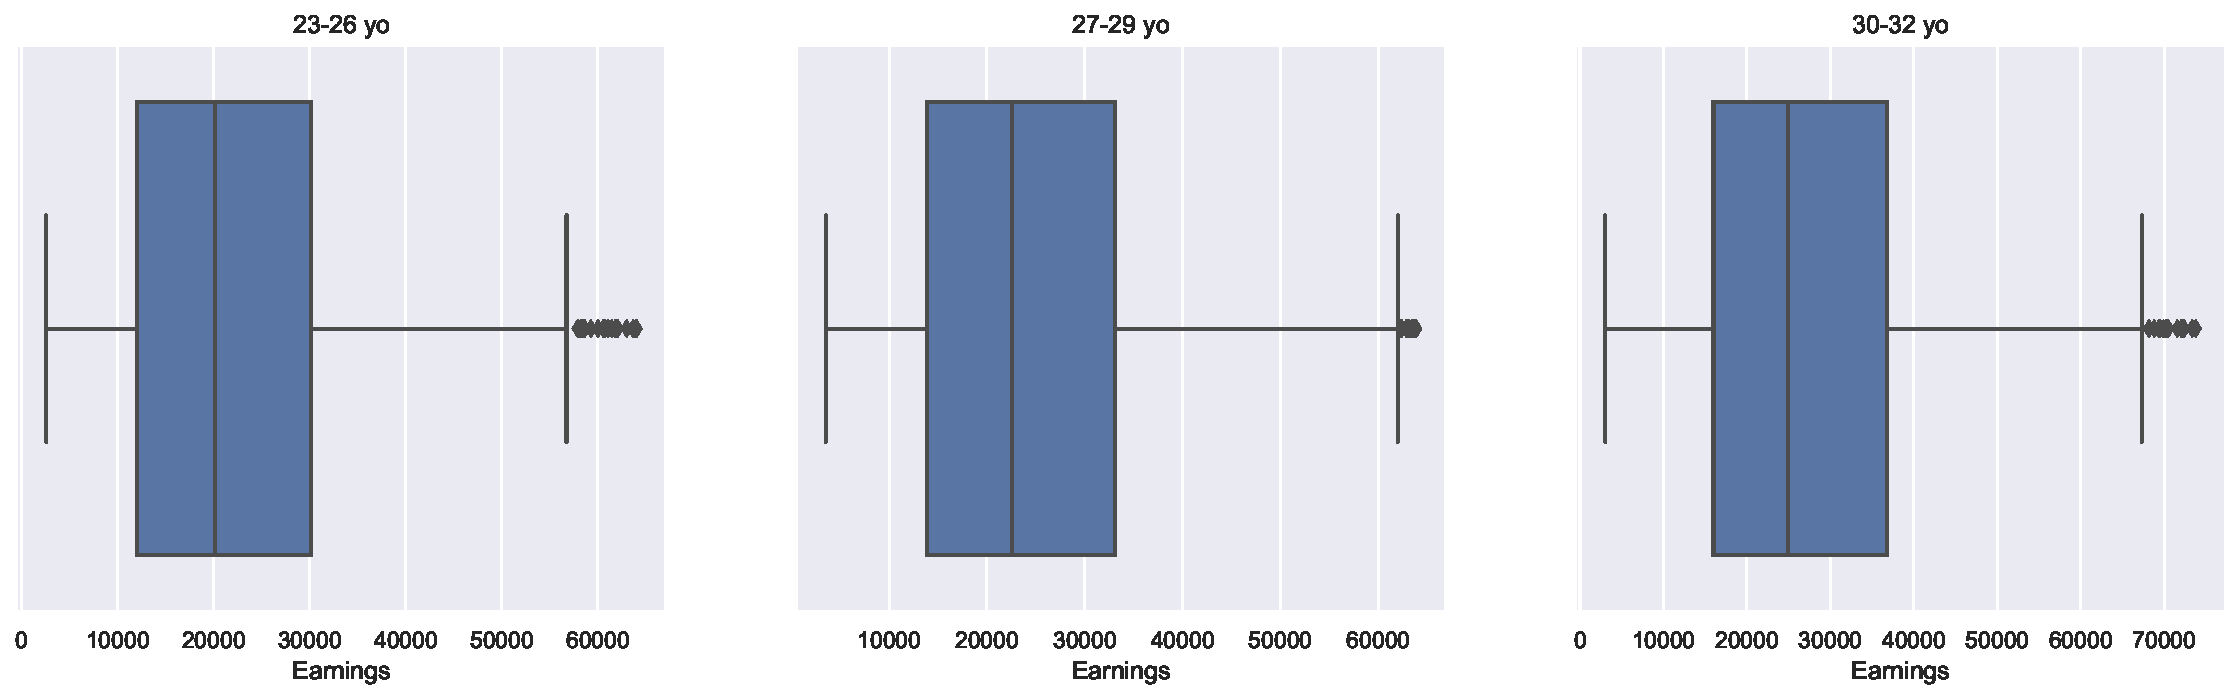
\includegraphics[scale=0.37]{boxplot1.pdf}
	\caption{Wykresy pudełkowe dla trzech grup wiekowych}
	\end{center}
\end{figure} 

\noindent Wartości średnie wynagrodzeń rosną wraz z numerem grupy, który jest warunkowany wiekiem. Może to mieć związek z większym doświadczeniem pracownika. Bardzo wysokie odchylenie standardowe w stosunku do średniej (około $ 60 \% $) oznacza, że w każdej grupie wiekowej są ogromne dysproporcje zarobków. Porównując wartości minimalne i maksymalne otrzymujemy różnicę rzędu $80$ tysięcy. Uwzględniając fakt, że średnie są zawsze większe od percentyla $50\%$ o około $2,5$ tysiąca ($12\%$), można wywnioskować, że rozbieżność płac jest spowodowana jednostkami, które zarabiają znacznie więcej od pozostałych. Zgadza się to z wykresami pudełkowymi. Na każdym z nich można zaobserwować wartości odstające z prawej strony. Co więcej, owe wykresy zostały sporządzone z danych po winsoryzacji. Zastąpienie skrajnych danych najbliższymi wartościami spowodowało wyraźne spadki wartości średnich zarobków, zwłaszcza w pierwszej grupie. Świadczy to o nielicznych relatywnie wysokich obserwacjach, które zawyżają statystyki opisowe. \\ 


\noindent Dane są zgodne z zasadą Pareto. Sumując ze sobą $20\%$ największych wynagrodzeń, a następnie dzieląc je przez zarobki wszystkich pracowników otrzymamy $77\%$, czyli wartość zbliżoną do progu $80\%$. \\ 


\noindent Dla porównania, średnie zarobki w Polsce na przełomie lat 1988/1989 wynosiły około 480 dolarów rocznie, czyli ponad 50 razy mniej.





\subsection{Analiza rozkładu danych}
\noindent

\begin{figure}[H]
	\begin{center}
	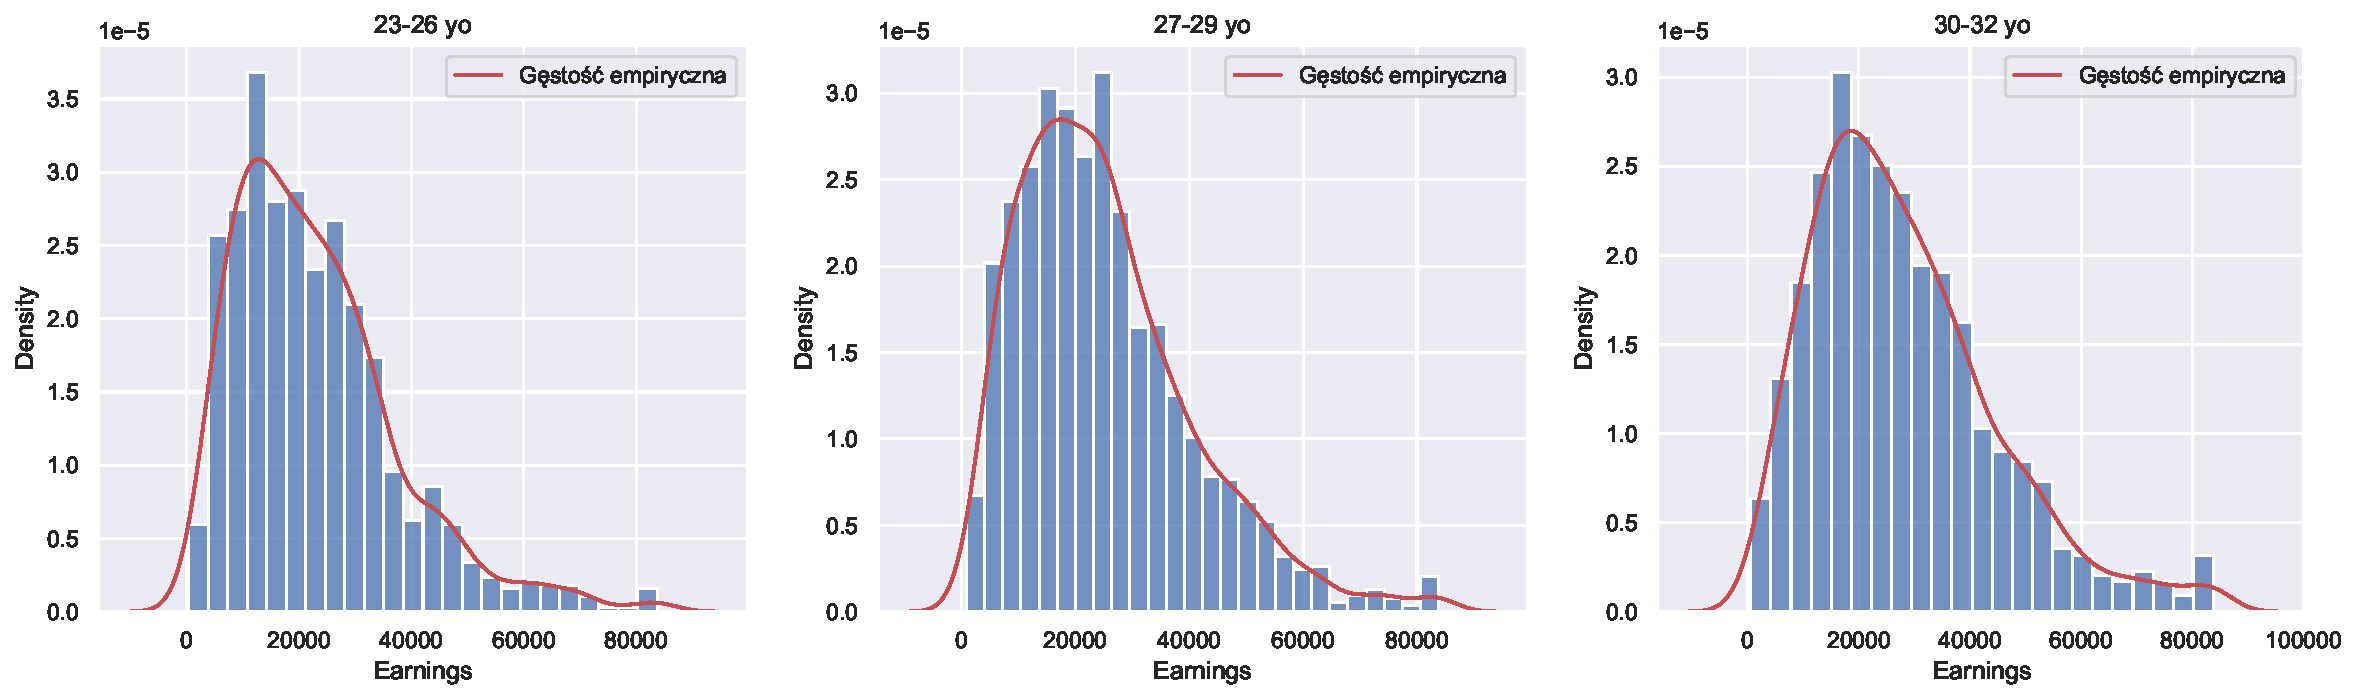
\includegraphics[scale=0.37]{histogramy1.pdf}
	\caption{Histogramy dla trzech grup wiekowych}
	\end{center}
\end{figure}

\noindent Histogramy nie oddają w pełni różnic otrzymanych w tabeli. Mają zbliżone kształty, a wcześniej wykazane dysproporcje obrazują ostatnie słupki. Najwięcej pracowników zarabiających w okolicy 80 tysięcy należy do najstarszej grupy wiekowej, co powoduje zawyżenie statystyk opisowych. Istotną różnicą są wyraźne dominanty w pierwszej i trzeciej grupie, podczas gdy środkowy wykres jest bardziej wypłaszczony. Może to świadczyć o istnieniu standardowych pensji dla pracowników w przedziałach wiekowych 23-26 i 30-32 lat. Innym wyjaśnieniem tego zjawiska może być proces nabywania doświadczenia. W drugiej grupie wiekowej znajdują się osoby, które otrzymały już podwyżkę oraz osoby, które nadal są w trakcie szkolenia i mają awans przed sobą.

\begin{figure}[H]
	\begin{center}
	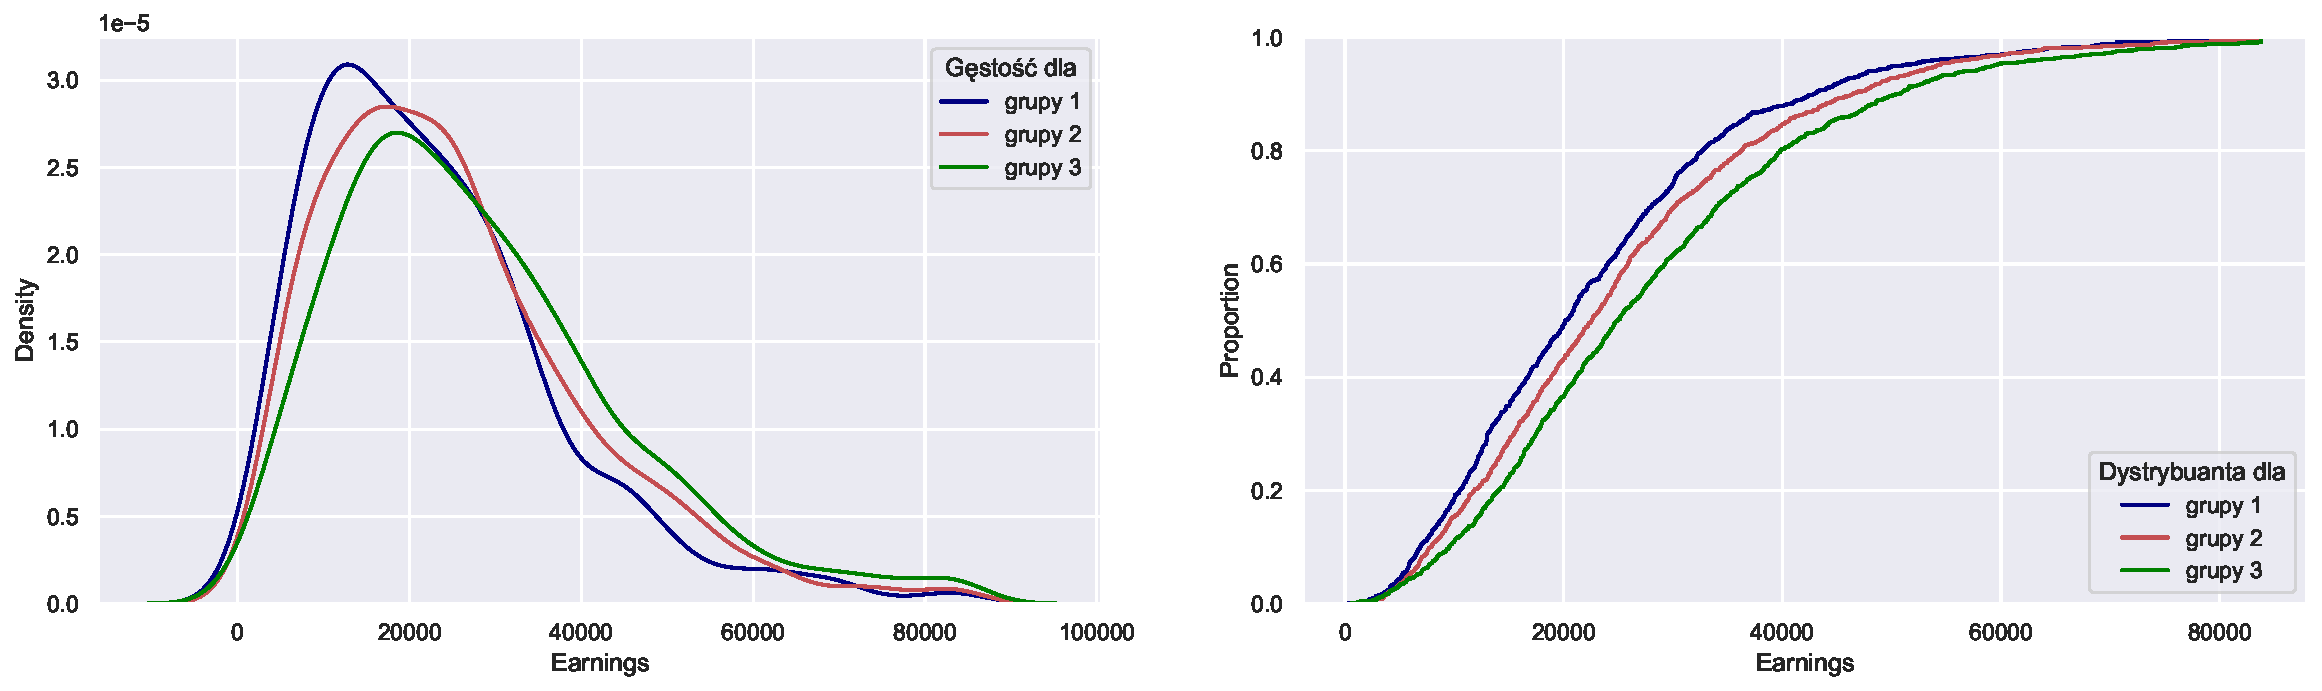
\includegraphics[scale=0.37]{gd1.pdf}
	\caption{Porównanie gęstości i dystrybuant dla trzech grup wiekowych}
	\end{center}
\end{figure}

\noindent Zbliżone kształty wykresów sugerują, że dane z trzech grup wiekowych mają ten sam rozkład, ale z różnymi parametrami. Wygląd krzywych wskazuje na rozkład gamma z dwoma parametrami.


\begin{figure}[H]
	\begin{center}
	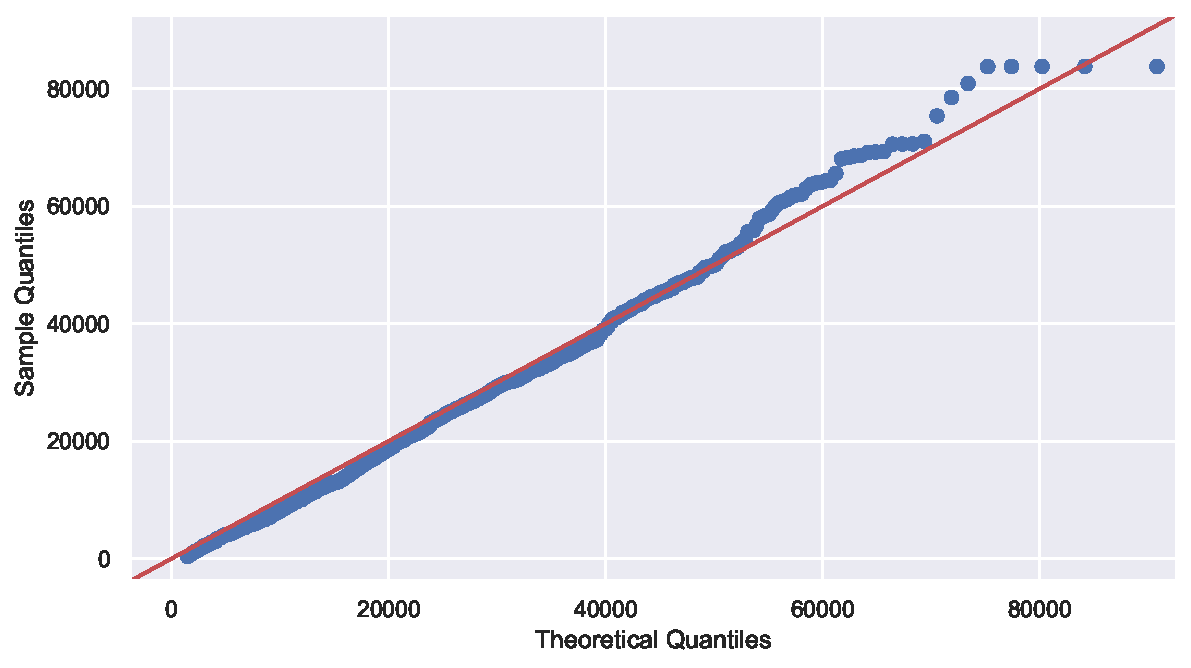
\includegraphics[scale=0.37]{qqplot1.pdf}
	\caption{Wykres kwantylowy dla pierwszej grupy}
	\end{center}
\end{figure}

\noindent Wykres kwantylowy został wykonany z argumentem Gamma$(3,0,8000)$. Dane układają się wzdłuż czerwonej linii nachylonej do osi OX pod kątem $45^{\circ}$, zatem rozkład zarobków pierwszej grupy wiekowej jest zbliżony do rozkładu Gamma$(3,8000)$.








\section{Drugi zestaw danych}
\subsection{Wprowadzenie}
\noindent Dane zostały pozyskane ze strony internetowej \url{https://vincentarelbundock.github.io/Rdatasets/datasets.html}. Dotyczą zarobków w Stanach Zjednoczonych w $1982$ roku. Składają się z $595$ obserwacji. Każdej z nich przypisano $12$ zmiennych, w tym miesięczną pensję w dolarach oraz informację o stanie małżeńskim pracownika.


\begin{figure}[H]
	\begin{center}
	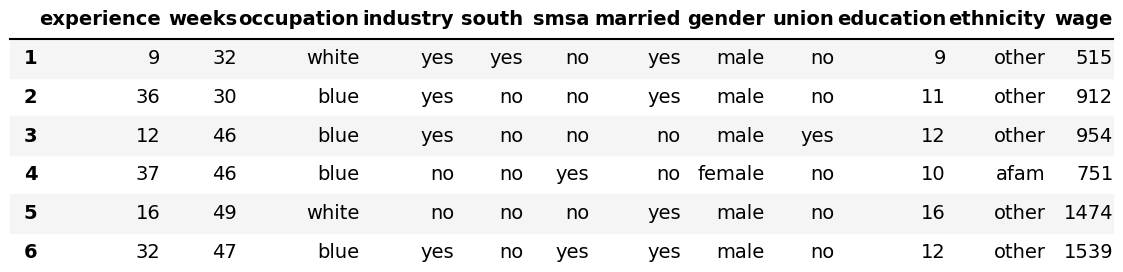
\includegraphics[scale=0.5]{head2.png}
	\caption{Przykładowe dane}
	\end{center}
\end{figure}



\subsection{Analiza danych}
\noindent Efektywne badanie korelacji między pensją a stanem małżeńskim wymaga rozpatrywania obu tych grup osobno. 

\begin{figure}[H]
	\begin{center}
	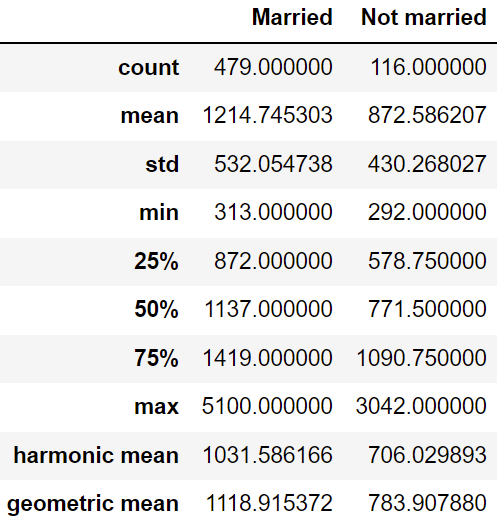
\includegraphics[scale=0.6]{compared2.png}
	\caption{Statystyki opisowe dla obu stanów cywilnych}
	\end{center}
\end{figure}

\begin{figure}[H]
	\begin{center}
	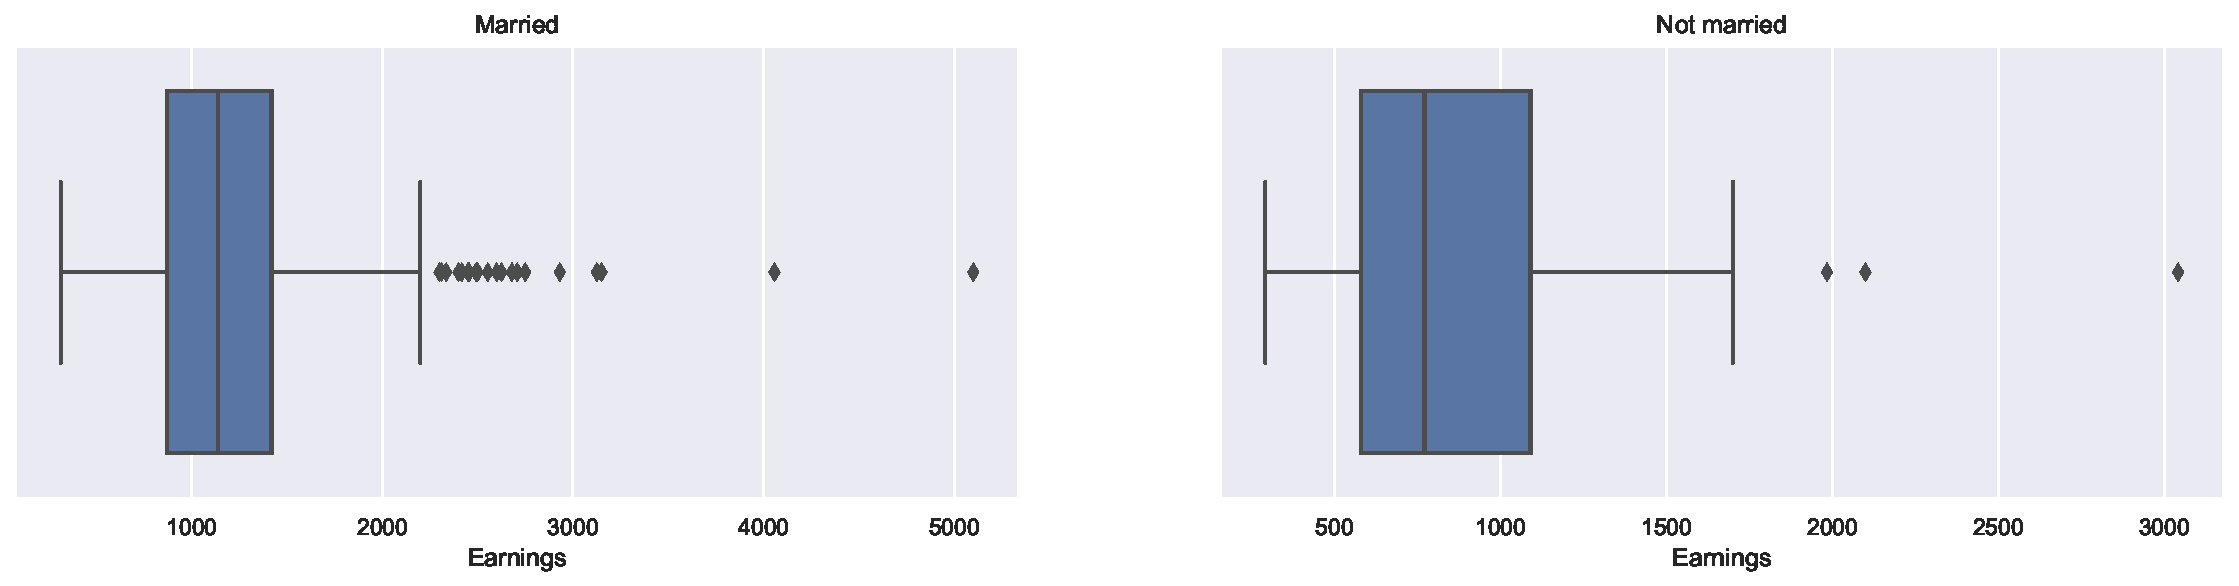
\includegraphics[scale=0.4]{boxplot2.pdf}
	\caption{Wykres pudełkowy dla obu stanów cywilnych}
	\end{center}
\end{figure}

\noindent Zdecydowaną większość obserwacji stanowią osoby w związku małżeńskim. Średnie wynagrodzenie dla tej grupy osób jest zdecydowanie wyższe. Może to mieć związek z wiekiem, a co za tym idzie, z większym doświadczeniem zawodowym. Innym powodem może być po prostu chęć zabezpieczenia rodziny finansowo. Ponownie możemy zaobserwować bardzo wysokie odchylenie standardowe w stosunku do średniej ($ 43\%$ i $49 \% $). To oznacza, że w obu grupach występują dysproporcje zarobków. Zgodnie z wykresami pudełkowymi, są to pojedyncze obserwacje, które znacznie zawyżają statystyki opisowe. 




\subsection{Analiza rozkładu danych}

\begin{figure}[H]
	\begin{center}
	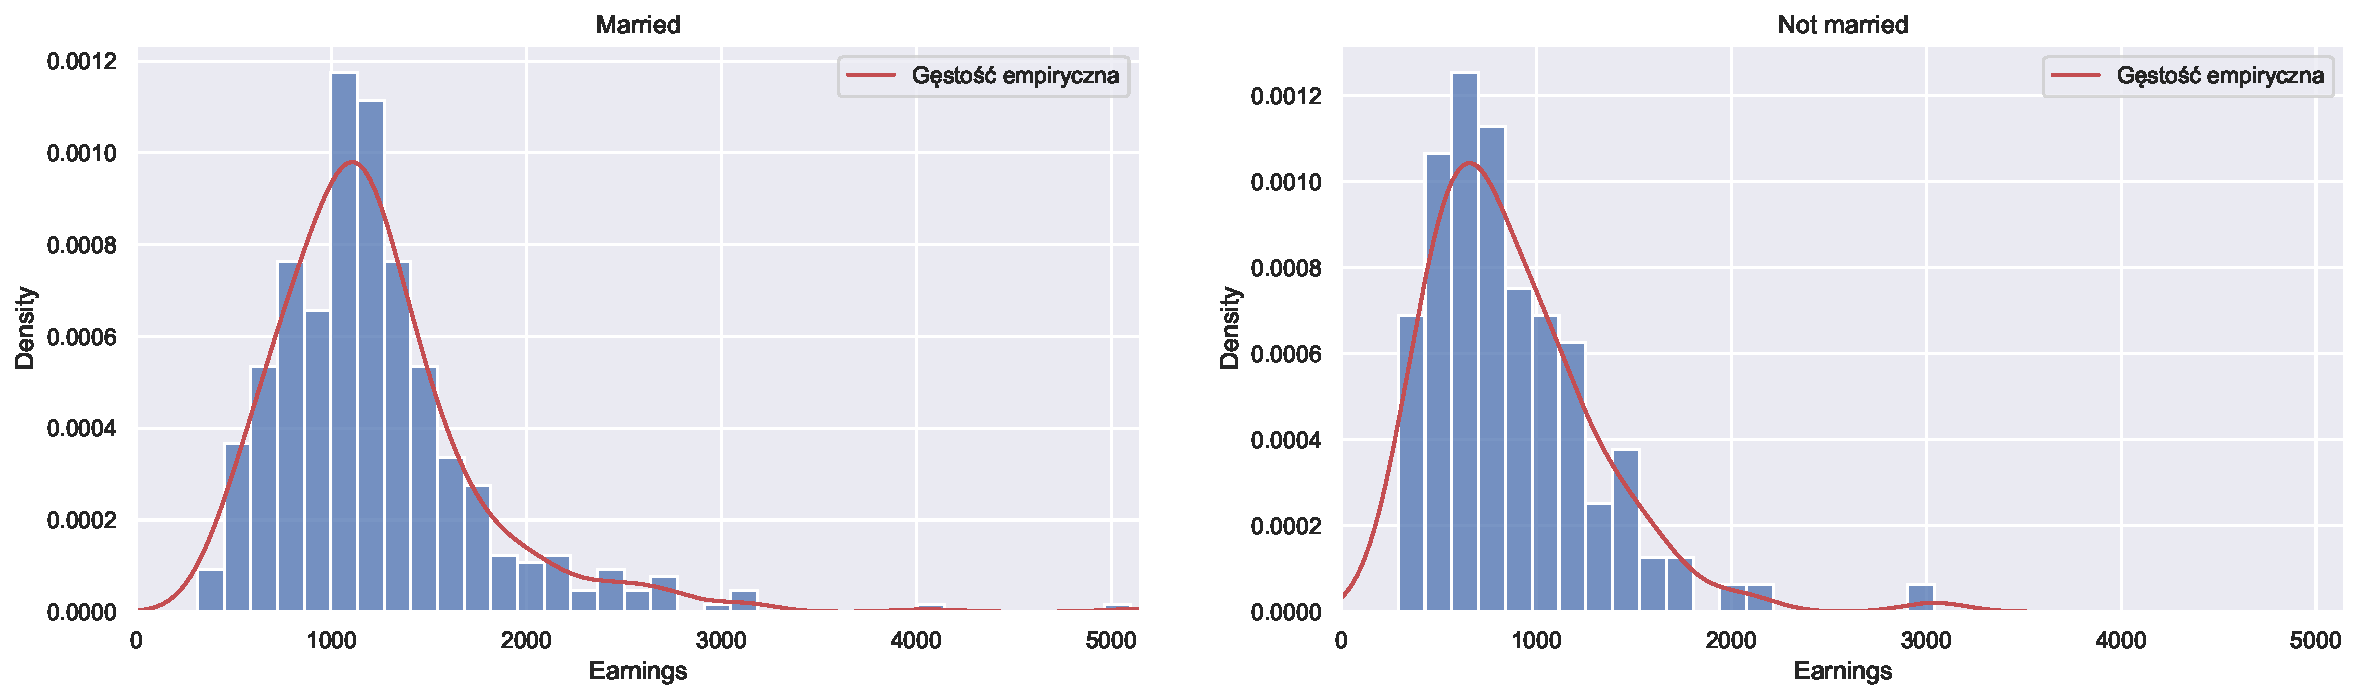
\includegraphics[scale=0.37]{histogramy2.pdf}
	\caption{Histogramy dla obu stanów cywilnych}
	\end{center}
\end{figure}

\noindent Histogramy obrazują wyraźne przesunięcie dominanty. Płace dla osób w związku małżeńskim skupiają się powyżej 1000 dolarów, a u osób stanu wolnego poniżej tej wartości. Co więcej, bardzo dobrze widać dlaczego odchylenie standardowe w drugiej grupie jest mniejsze. Praktycznie nie występują obserwacje powyżej 2200 dolarów, a maksymalna wartość wynosi w przybliżeniu 3000 dolarów.

\begin{figure}[H]
	\begin{center}
	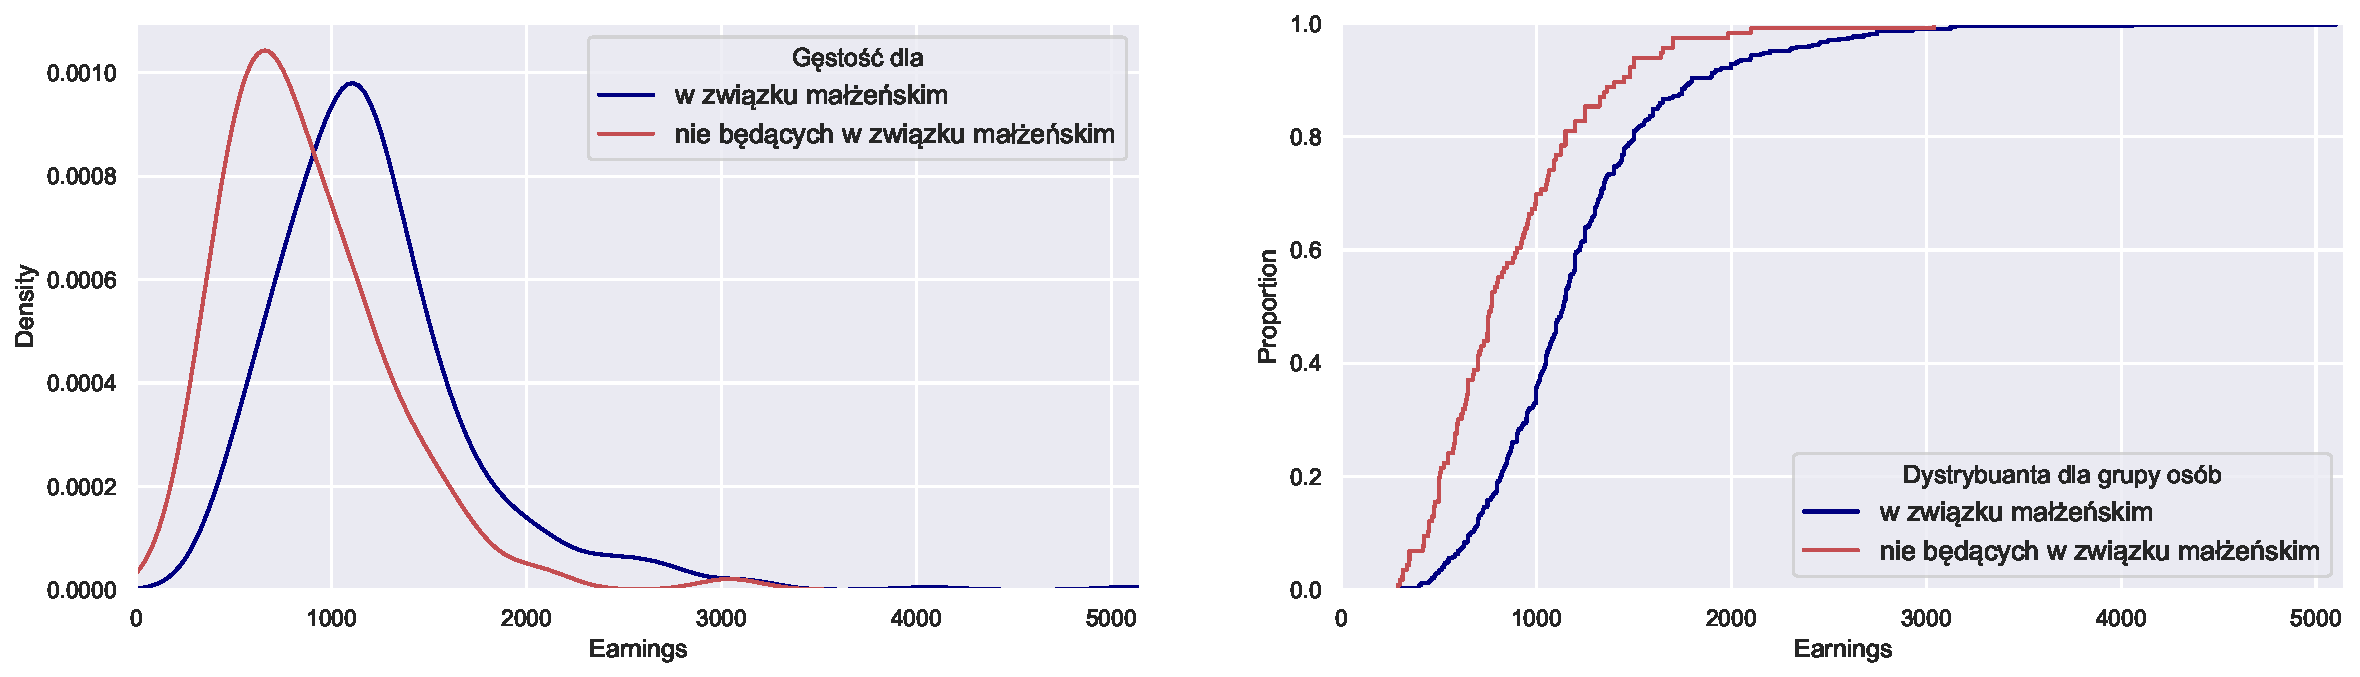
\includegraphics[scale=0.37]{gd2.pdf}
	\caption{Porównanie gęstości i dystrybuant dla obu stanów cywilnych}
	\end{center}
\end{figure}

\noindent Zbliżone kształty wykresów sugerują, że zarobki dla obu stanów cywilnych mają ten sam rozkład, ale z różnymi parametrami.
	


\section{Podsumowanie}
\noindent Poznane metody statystyczne pozwoliły na dogłębną analizę danych rzeczywistych. Odpowiedni podział i badanie obserwacji pod wieloma względami odpowiedziały na pytanie jak poszczególne czynniki wpływają na pensję pracownika. Powyższa praca również pokazała jak ważne jest kompleksowe podejście do tematu. Wizualizacja danych oraz takie procesy jak winsoryzacja lub średnia ucinana mają ogromne znaczenie w procesie wyciągania wniosków.


\end{document}